\documentclass[12pt, a4paper]{article}

\usepackage[utf8]{inputenc}
\usepackage[spanish]{babel}
\usepackage{titling}
\usepackage[left=2cm,right=2cm,top=2cm,bottom=2cm]{geometry}
\usepackage{enumerate}
\usepackage{amsmath}
\usepackage{graphicx}

\usepackage{listings}%-para agregar codigo-
\usepackage[usenames,dvipsnames]{color}
\usepackage{color}%------------------------

%---------------------importar codigo desde archivos cpp----------------------------
\lstloadlanguages{C++}
\lstnewenvironment{code}
	{%\lstset{	numbers=none, frame=lines, basicstyle=\small\ttfamily, }%
	 \csname lst@SetFirstLabel\endcsname}
	{\csname lst@SaveFirstLabel\endcsname}
\lstset{% general command to set parameter(s)
	language=C++, basicstyle=\small\ttfamily, keywordstyle=\slshape,
	emph=[1]{tipo,usa}, emphstyle={[1]\sffamily\bfseries},
	morekeywords={tint,forn,forsn},
	basewidth={0.47em,0.40em},
	columns=fixed, fontadjust, resetmargins, xrightmargin=5pt, xleftmargin=15pt,
	flexiblecolumns=false, tabsize=2, breaklines,	breakatwhitespace=false, extendedchars=true,
	numbers=left, numberstyle=\tiny, stepnumber=1, numbersep=9pt,
	frame=l, framesep=3pt,
    basicstyle=\ttfamily,
    keywordstyle=\color{blue}\ttfamily,
    stringstyle=\color{magenta}\ttfamily,
    commentstyle=\color{RedOrange}\ttfamily,
    morecomment=[l][\color{OliveGreen}]{\#}
}

\lstdefinestyle{C++}{
	language=C++, basicstyle=\small\ttfamily, keywordstyle=\slshape,
	emph=[1]{tipo,usa,tipo2}, emphstyle={[1]\sffamily\bfseries},
	morekeywords={tint,forn,forsn},
	basewidth={0.47em,0.40em},
	columns=fixed, fontadjust, resetmargins, xrightmargin=5pt, xleftmargin=15pt,
	flexiblecolumns=false, tabsize=2, breaklines,	breakatwhitespace=false, extendedchars=true,
	numbers=left, numberstyle=\tiny, stepnumber=1, numbersep=9pt,
	frame=l, framesep=3pt,
    basicstyle=\ttfamily,
    keywordstyle=\color{blue}\ttfamily,
    stringstyle=\color{magenta}\ttfamily,
    commentstyle=\color{RedOrange}\ttfamily,
    morecomment=[l][\color{OliveGreen}]{\#}
}

\def\nbtitle#1{\begin{Large}\begin{center}\textbf{#1}\end{center}\end{Large}}
\def\nbsection#1{\section{#1}}
\def\nbsubsection#1{\subsection{#1}}
\def\nbcoment#1{\begin{small}\textbf{#1}\end{small}}
\newcommand{\comb}[2]{\left( \begin{array}{c} #1 \\ #2 \end{array}\right)}
\def\complexity#1{\texorpdfstring{$\mathcal{O}(#1)$}{O(#1)}}
 \newcommand\cppfile[2][]{
\lstinputlisting[style=C++,linerange={#1}]{#2}
}
%%------------------------------------------------------------------------------

\newcommand{\subtitulo}[1]{\begin{center}\textbf{#1}\end{center}}

\title{\textbf{Programación Dinámica}}
\author{Wilmer Emiro Castrillón Calderón}

\graphicspath{{../}}
\newcommand*\lstinputpath[1]{\lstset{inputpath=#1}}
\lstinputpath{../}

\begin{document}
	\maketitle
	
	%<*Capitulo>
	
	\section{Introducción a la programación dinámica}
	
	La programación dinámica es una metodología utilizada para reducir la complejidad computacional a un
	algoritmo, es usada principalmente para resolver problemas de optimización,
	se basa en la estrategia \textit{divide y vencerás}, consiste en tomar un problema complejo y dividirlo 
	sucesivamente en sub-problemas mas pequeños hasta llegar a un caso base, y partir de ahí empezar a construir la
	solución de cada sub-problema, hasta llegar a una solución global. Durante la búsqueda de soluciones
	se utiliza tablas de memorización, en la cuales se irá guardando la solución óptima de cada sub-problema.
	Como abreviatura a programación dinámica vamos a usar dp, pues son sus siglas en ingles.
	
	Los problemas que pueden ser resueltos utilizando programación dinámica presentan tres condiciones básicas:
	\begin{enumerate}[1.]
		\item El problema se puede dividir en sub-problemas, y estos a su vez en más sub-problemas, y así hasta llegar
				a uno o múltiples casos base.
		\item La solución óptima de cada sub-problema depende de la solución óptima de cada uno de sus
				propios sub-problemas, entonces cumple con el principio de optimalidad de Bellman.
		\item Se presenta superposición de problemas, es decir, existen sub-problemas que aparecen múltiples veces
		 		a lo largo de la búsqueda de la solución general. Aunque como tal no es obligatorio, es la razón 
		 		principal que le permite tener menor complejidad computacional.
	\end{enumerate}
	
	\subtitulo{Ejemplo inicial.}
	
	El ejemplo básico más usado es con la sucesión de Fibonacci, esta comienza con los números 0 y 1, y a partir
	de estos dos números iniciales los siguientes son la suma de los dos anteriores, entonces los primeros
	números de Fibonacci son:
	\begin{center} $0, 1, 1, 2, 3, 5, 8, 13, 21, 34, 55, 89, ..... $ \end{center}
	
	Ahora se buscará la manera de calcular y guardar en un vector los primeros $n$ números de la sucesión 
	eficientemente, de tal forma que la posición i-esima del vector corresponda al número i-esimo de la sucesión.
	Para solucionar el problema con dp primero debemos identificar los sub-problemas, es decir dividir el problema en
	partes mas pequeñas, en este caso obtenemos la siguiente formula recursiva:\\
	\begin{center}
		$fibo(n) = 	
			\begin{cases}
				n & \text{if $n\le 1$}\\
				fibo(n-1) + fibo(n-2) & \text{if $n\ge 2$}
		\end{cases}	$\\
	\end{center}
	
	Para implementar dp surgen dos enfoques: Top-Down y Buttom-Up, vamos a resolver este ejemplo usando los dos.\\
	
	\textbf{Buttom-Up}\\
	En este enfoque vamos a ir recorriendo la tabla de memorización mientras la llenamos, comenzando desde los
	casos base de la formula recursiva y a partir de ahí ir calculando y guardando los demás resultados en la
	tabla. En este enfoque primero se calcula el resultado de todos los subproblemas antes de dar alguna solución 
	global. Para este ejercicio comenzamos llenando en un vector \textit{v} los casos
	base: \textit{v[0] = 0; v[1] = 1;} y luego llenamos el resto del vector según nos indica la formula
	recursiva: \textit{v[i] = v[i-1] + v[i-2]}, de tal forma que \textit{v[i-1]} y \textit{v[i-2]} son valores
	que se han calculado antes y ademas $v[x] = fibo(x)$. A continuación se muestra el ejemplo en C++ calculando
	los primero 45 números de la sucesión:
	\cppfile[7-12]{Programacion_dinamica/codigos/fibo.cpp}
	Aunque en este enfoque no utilizamos llamados recursivos, puede resultar mas difícil de implementar,
	pues por lo general es menos intuitivo.\\
	
	\textbf{Top-Down}\\
	A diferencia del anterior enfoque en este vamos a utilizar llamados recursivos, en los cuales se irá guardando
	los resultados en la tabla de memorización mientras se calculan, y así evitar que se realice dos veces el
	mismo llamado recursivo. Es decir se calcula el resultado solo de los subproblemas que sean necesarios para 
	dar alguna solución global, a diferencia del Buttom-Up donde se calculaban primero todos los
	subproblemas antes de poder dar alguna solución. En este enfoque se hace mas notorio la importancia de la tabla 
	de memorización, veamos la eficiencia del algoritmo si dejamos únicamente la formula recursiva, el código seria 
	el siguiente:
	\cppfile[14-19]{Programacion_dinamica/codigos/fibo.cpp}
	Si ejecutamos este código para $fibo(6)$ obtenemos el siguiente arbol de recursión:\\
	\begin{center}
		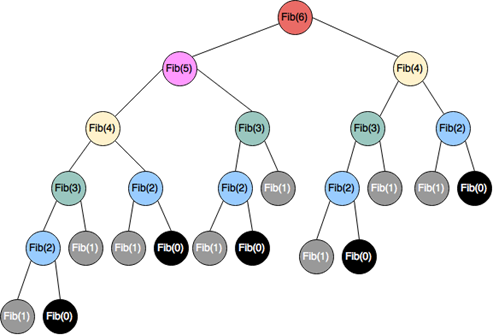
\includegraphics[scale=0.92]{Programacion_dinamica/imagenes/arbol_recursion}
	\end{center}
	
	Se puede observar que se realizan múltiples llamados repetidos, $fibo(4)$ se repite 2 veces, $fibo(3)$
	3 veces, $fibo(2)$ 5 veces, $fibo(1)$ 8 veces y $fibo(0)$ 5 veces, resultan bastantes llamados recursivos
	solamente para encontrar $fibo(6)$, esta solución tiene ¡una complejidad exponencial!, en números pequeños
	no es muy notorio pero cuando intentamos encontrar $fibo(42)$ o $fibo(45)$ el tiempo de ejecución se hace
	muy alto, entonces para mejorar el tiempo se debe implementar una tabla de memorización, en la cual se guardara
	el resultado de cada llamado recursivo, ademas se debe agregar un condicional al inicio del método preguntando
	si la solución de ese sub-problema ya fue encontrada, en tal caso se devuelve el valor guardado, sino se calcula
	y se guarda, en este ejemplo la tabla comienza llena con -1, un valor que nunca es usado en la solución, de 
	tal forma que si una posición es igual a -1 entonces se debe calcular.
	\cppfile[24-31]{Programacion_dinamica/codigos/fibo.cpp}
	Este ejercicio resulta muy trivial, se puede resolver facilmente sin pensar en dp, ahora se mostraran
	problemas en los cuales se hace necesario utilizar dp para dar una solución eficiente.
	
	\subtitulo{Recorrido óptimo en una matriz.}
	
	Teniendo una matriz de $n$ x $m$ con números enteros, se quiere conocer la suma maxima que se puede obtener
	recorriendo la matriz, comenzando desde la esquina superior-izquierda y terminando en la esquina inferior-derecha,
	realizando únicamente pasos hacia la derecha y abajo, por ejemplo:\\
	\begin{center}
		\begin{tabular}{|l|l|l|}
			\hline
			5  &6 &4 \\ \hline
			3  &8  &5 \\ \hline
			2 &11 &15 \\ \hline
			5 &2  &17 \\ \hline
		\end{tabular}
	\end{center}
	El camino óptimo es 5-6-8-11-15-17 y la suma es 62.\\
	
	Este es un problema de optimización, a simple vista la solución consistiría de siempre ir a la casilla adyacente
	con mayor valor, pero no siempre es el mejor camino, por ejemplo con la siguiente matriz:
	\begin{center}
		\begin{tabular}{|l|l|l|l|}
		 	\hline
			1  & 12 & 4  & 9 \\ \hline
			6  & 5  & 21 & 15 \\ \hline
			35 & 18 & 8  & 10 \\ \hline
			12 & 2  & 4  & 15 \\ \hline
		\end{tabular}
	\end{center}
	No es una solución óptima ir a la siguiente casilla con mayor valor, pues haciendo esto se tendría el siguiente
	camino 1-12-5-21-15-10-15 con un acumulado de 79, en cambio el camino 1-6-35-18-8-10-15 tiene un acumulado de 93,
	entonces con la anterior estrategia no siempre se obtiene el camino óptimo. En este problema es necesario realizar
	una toma de decisiones, pues existen múltiples opciones de caminos, y se necesita encontrar el conjunto de
	decisiones que permita llegar a un resultado optimo, una solución inicial puede ser con BackTraking pero esta 
	tendría complejidad exponencial O($2^{n}$), por lo tanto se necesita utilizar otro enfoque.\\
	
	Este problema se puede resolver con programación dinámica, pues se puede encontrar la solución general a partir de 
	la solución de sub-problemas más pequeños, supongamos que tenemos una matriz $T$ de tamaño $n$ x $m$ a la cual se 
	va a calcular la suma de su recorrido óptimo, para facilidad se indexara desde 1 tomando la esquina superior
	izquierda como T[1][1], para encontrar el camino óptimo hasta T[n][m](ultima casilla) es necesario primero 
	encontrar el óptimo de T[n-1][m] y T[n][m-1], pues para llegar a T[n][m] hay dos opciones, llegar por arriba
	(equivalente a tomar la decisión ir-abajo desde T[n-1][m]) o llegar por la izquierda (equivalente a tomar la 
	decisión ir-derecha desde T[n][m-1]), entonces la solución general sera \textit{T[n][m] + máximo entre(camino 
	óptimo hasta T[n-1][m], camino óptimo hasta T[n][m-1])}, y a su vez el óptimo para ellos se calcula de manera
	similar, el  optimo para llegar hasta T[n-1][m] es \textit{T[n-1][m] + máximo entre(camino óptimo hasta T[n-2][m],
	camino óptimo hasta T[n-1][m-1])} y  de manera similar para T[n][m-1], de esta forma se puede dividir el problema 
	en sub-problemas.\\
	
	Ahora ya se puede empezar a construir una formula recursiva, llamaremos $i$ a la posición en fila y $j$ a la 
	posición en columna, entonces $f(i,j)$ devolverá el valor del recorrido optimo desde T[1][1] hasta T[i][j], 
	ahora se deben establecer los casos base, entonces si $i$ y $j$ son iguales a 1 entonces el resultado es 
	T[1][1](se encuentra en el punto inicial), si solo $i$ es 1 entonces el resultado es \textit{T[1][j] + f(1,j-1)},
	solo se puede llegar a T[1][j] desde su izquierda, pues desde arriba estaría afuera de la matriz, si solo $j$ 
	es 1 entonces de manera similar se tiene como resultado \textit{T[i][1] + f(i-1,1)}, ahora ya se tienen los 
	casos base y se puede construir la formula recursiva:
	\begin{center}
		$f(i, j) = 	
		\begin{cases}
			T[1][1] & \text{if $i,j = 1$}\\
			T[1][j] + f(1, j-1) & \text{if $i = 1$}\\
			T[i][1] + f(i-1, 1) & \text{if $j = 1$}\\
			T[i][j] + mayor(f(i-1, j), f(i, j-1)) & \text{if $i,j \neq 1$}
		\end{cases}
	$\\
	\end{center}
	Realzando manualmente la función recursiva se puede tener mas claridad. El caso $f(1,1)$ indica que la solución
	es el elemento en la primera casilla, la solución para la primera fila sera la sumatoria de los elementos desde 
	la primera casilla hasta la columna correspondiente, ese es el único camino posible, de similar manera ocurre
	con la primera columna (figura 1), para los demás casos se abren dos opciones, llegar desde arriba o llegar desde
	la izquierda (figura 2), la formula indica tomar el de mayor valor, de esta manera mientras se avanza se ira 
	seleccionando el mejor camino hasta llegar a la ultima casilla.\\
	
	\begin{figure}[!htb]
		\minipage{0.33\textwidth}
			\centering
			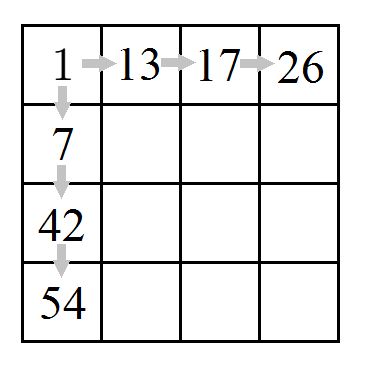
\includegraphics[scale=0.4]{Programacion_dinamica/imagenes/matriz1}
			\caption{}%\label{fig:awesome_image1}
		\endminipage
		\minipage{0.33\textwidth}
			\centering
			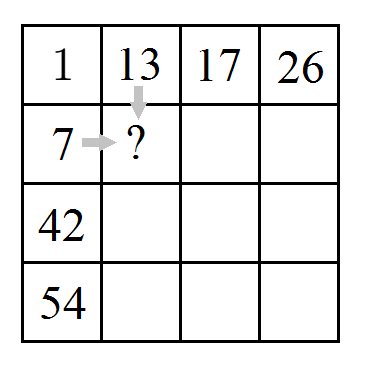
\includegraphics[scale=0.4]{Programacion_dinamica/imagenes/matriz2}
			\caption{}
		\endminipage
		\minipage{0.33\textwidth}
			\centering
			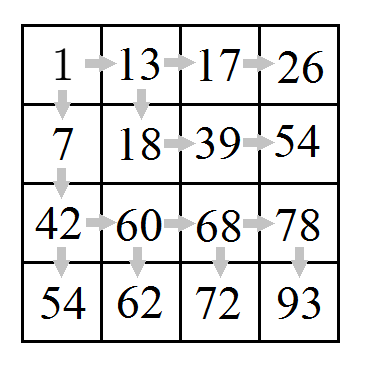
\includegraphics[scale=0.4]{Programacion_dinamica/imagenes/matriz3}
			\caption{}%\label{fig:awesome_image1}
		\endminipage
	\end{figure}
	
	Para terminar el dp es necesario agregar la tabla de memorización, pues aplicar la formula directamente resultaría
	en un algoritmo de complejidad exponencial, como tabla de memorización se usara otra matriz de igual tamaño,
	esta se llamara memo y guardara las soluciones, es decir, que en memo[i][j] se guardara el acumulado óptimo para 
	ir desde T[1][1] hasta T[i][j], en otras palabra memo[i][j] = $f(i,j)$, ahora se puede solucionar el problema 
	usando cualquiera de los dos enfoques de dp, para usar Top-Down solamente se agrega la tabla de memorización 
	a la formula recursiva, resultando en la siguiente función(recordar que en C++ se indexa desde 0):
	\cppfile[9-17]{Programacion_dinamica/codigos/matriz.cpp}
	
	para conocer el resultado solo se debe imprimir $f(n-1, m-1)$. para la solución con Buttom-Up se debe recorrer 
	la matriz y llenarla según la formula recursiva, se debe comenzar con los casos base antes de calcular lo demás, 
	esto resultaría en la siguiente función:
	\cppfile[19-31]{Programacion_dinamica/codigos/matriz.cpp}
	De esta forma para conocer la solución se debe imprimir memo[n-1][m-1]. La complejidad algorítmica resultante
	es O($n*m$), resultando mejor que un algoritmo de complejidad exponencial utilizando fuerza bruta.\\
	
	\section{Sub-SetSum}
	
	También conocido como suma de subconjuntos, el problema consiste en que a partir de un conjunto de números enteros
	$V$, encontrar si es posible que otro número $n$ sea el resultado de la suma de los elementos de algún
	subconjunto de $V$, por ejemplo con el conjunto $V$={1, 2, 5} es posible sumar 7 usando el subconjunto \{2, 5\},
	con este conjunto $V$ seria posible sumar \{1, 2, 3, 5, 6, 7, 8\}.\\
	
	Utilizando un algoritmo de BackTraking para probar todos los posibles subconjuntos se obtendría una complejidad
	O($2^{n}$), siendo bastante alta aun para rango pequeños. Este problema puede ser resuelto usando dp, se puede
	reescribir el numero $n$ como: $n=V[k_{1}]+x_{1}$, con $V[k_{1}]$ como algún numero en $V$, de manera similar se
	puede reescribir $x_{1}$ como $x_{1}=v[k_{2}]+x_{2}$ y así sucesivamente hasta encontrar $x_{n}=v[k_{n}]+0$, de 
	esta manera si se toma cada elemento de $V$ que fue utilizado, se podría encontrar el subconjunto:
	${v[k_{1}],v[k_{2}],...,v[k_{n}]}$ el cual sumando todos sus elementos obtenemos $n$, en general se deberá probar
	para cada elemento en $V$ si puede pertenecer a algún subconjunto que sume $n$.\\
	
	En este problema el resultado deberá ser 'verdadero' o 'falso', mostrando si es posible sumar $n$ con algún 
	subconjunto, con los sub-problemas establecidos se puede ahora definir los casos base, si en algún momento 
	se llega a $x_{n}=0$ entonces la solución global sera 'verdadero'(se encontró una solución, entonces es posible 
	sumar $n$), pero si en algún momento usamos todos los elementos en $V$ y aun $x_{n}>0$, o 
	en algún momento se llega a $x_{n}<0$ entonces la solución en ese sub-problema sera 'falso', entonces se tiene la
	siguiente función recursiva(siendo 1 verdadero, y 0 falso):
	\begin{center}
		$f(n, k) = 	
		\begin{cases}
			1 & \text{if n = 0}\\
			0 & \text{if n $<$ 0, k$>longitud( $V$)$}\\
			1 & \text{if f(n-V[k],k+1)=1}\\
			0 & \text{if $otro$}
		\end{cases}
		$\\
	\end{center}
	Con esta formula la solución sera igual a $f(n,0)$, para implementarla se debe hacer una tabla de memorización,
	la cantidad de columnas de la tabla debe ser por lo menos igual a la longitud del vector, y la cantidad 
	de filas por lo menos igual al resultado más grande que se puede obtener. Igualmente se llenara inicialmente con -1.
	\cppfile[24-33]{Programacion_dinamica/codigos/SubSetSum.cpp}
	
	Este problema también puede ser resuelto usando el enfoque Buttom-Up, donde se buscaría todas las posibles 
	sumas que se pueden formar con los números en $V$, se tomara $m$ como el tamaño de $V$ y por facilidad se usara 1 
	como indice inicial. Los subproblemas se podrían ver de la siguiente manera: la solución general incluye sumar el
	elemento $V[m]$ a todas las soluciones encontradas hasta $V[m-1]$, y este a su vez depende de encontrar $V[m-1]$
	y así sucesivamente hasta llegar a $V[1]$ que sera nuestro caso base, mas detalladamente la solución hasta $V[1]$ 
	es solamente él mismo, las soluciones hasta $V[2]$ es él mismo, $V[1]$ y la suma $V[1]+V[2]$, el conjunto de
	soluciones hasta ahora es \{$V[1]$, $V[2]$, $V[1]+V[2]$\}, ahora la solución hasta $V[3]$ sera 
	\{$V[1]$, $V[2]$, $V[3]$, $V[1]+V[2]$, $V[1]+V[3]$, $V[2]+V[3]$, $V[1]+V[2]+V[3]$\}, y así sucesivamente hasta 
	$V[m]$, descartando números repetidos.\\
	
	Por ejemplo sea $V$=\{3, 5 y 8\}, la solución hasta 3 es él mismo, el conjunto de soluciones hasta ahora es \{3\},
	la solución hasta 5 es él mismo y su suma con las soluciones anteriores, el conjunto de soluciones cambia a 
	\{3, 5, 8\}, y por ultimo incluyendo el 8 el conjunto resultante es: \{3, 5, 8, 11, 13, 16\}. Una posible
	implementación seria:\\
	\cppfile[8-21]{Programacion_dinamica/codigos/SubSetSum.cpp}
	
	En el anterior código se tienen dos ciclos, el primero recorriendo el vector $V$ y el segundo buscando las 
	soluciones anteriores para sumarles $V[i]$, como el caso base es cuando $i=0$ entonces se debe omitir el segundo
	ciclo cuando $i$ tiene este valor, ejecutando este código se obtendría todas las soluciones en la última columna,
	entonces si $memo[n][V.size()-1]$ es verdadero entonce si existe un sub-conjunto que sume $n$, en caso contrario
	no es posible.

	\section{Problema de la mochila(Knapsack problem)}
	
	Este es un problema clásico de programación dinámica, consiste en lo siguiente, hay una mochila que tiene una
	capacidad limitada de peso que puede contener, y hay un grupo de objetos, cada uno tiene un valor y peso, el
	objetivo consiste en llenar la mochila con los objetos de tal forma que no se exceda su capacidad de peso y 
	que el valor de los objetos que hay dentro de la mochila sea lo más alto posible. Por ejemplo:
	\begin{center}
		\begin{tabular}{|l|l|l|l|l|l|l|}
			\hline
			$i$  	&0 &1 &2 &3 &4 &5 \\ \hline
			$W_{i}$ &1 &2 &4 &5 &4 &2 \\ \hline
			$V_{i}$ &2 &7 &5 &9 &5 &3 \\ \hline
		\end{tabular}
	\end{center}
	Sea $N=6$ la cantidad de objetos, $C=10$ la capacidad de la mochila, $W_{i}$ el peso del i-ésimo objeto y 
	$V_{i}$ el valor del i-ésimo objeto, entonces las respuesta es 21, usando los objetos 0, 1, 3, 5 obtenemos un peso 
	10 con valor 21.\\
	
	Para cada objeto existen dos opciones, tomarlo o dejarlo, entonces para n objetos existen $2^{n}$ posibles 
	opciones, de todas ellas la solución será una configuración que no exceda el peso de la mochila y la suma de los
	objetos seleccionados sea el más alto, una solución probando todos los posibles casos tendrá complejidad 
	O($2^{n}$), la cual es bastante alta, mientras que una solución greddy no siempre va a funcionar.\\

	Sin embargo es posible reducir bastante la complejidad trabajando con programación dinámica, sea $x_{i}$ la 
	capacidad usada al estar en el i-ésimo objeto, iniciando con $i=0$ y $x_{i}=0$, se repite el siguiente proceso: 
	para cada objeto existe la decisión de no tomarlo y pasar al objeto $i+1$ con $x_{i+1}=x_{i}$ o tomarlo y pasar 
	al objeto $i+1$ con $x_{i+1}=x_{i}+W_{i}$ siempre y cuando $x_{i}+W_{i} \leq C$, es decir que no se exceda la 
	capacidad, entonces se puede escribir la siguiente función recursiva:
	\begin{center}
		$f(i, x) = 	
		\begin{cases}
			0 & \text{if } i = N\\
			max(f(i+1,x), f(i+1,x+W_{i}) + V_{i}) & \text{if } x+W_{i} \leq C \\
			f(i+1,x) & \text{if $otro$}
		\end{cases}
		$\\
	\end{center}
	
	Al programar esta función recursiva se obtendrá una complejidad de $O(2^{n})$, pero al agregar la tabla de 
	memorización la complejidad se reduce al tamaño de la tabla, quedado en $O(N*C)$, y finalmente se puede obtener 
	la siguiente implementación.
	\cppfile[9-17]{Programacion_dinamica/codigos/ProblemaMochila.cpp}
	
	
	
	\section{Bibliografia}
	
	http://trainingcamp.org.ar/anteriores/2017/clases.shtml.\\
	http://programacioncompetitivaufps.github.io/\\
	https://www.geeksforgeeks.org/dynamic-programming-subset-sum-problem/\\
	libro: competitive programming 3.\\

	%</Capitulo>
	
\end{document}



